\section{Results}

\subsection{Benchmark of values}

\begin{itemize}

  \item \textbf{Image: gain VS time for one single point. Overlay between
    experiment/daniels sim/our sim}

  \item comparison with previous values from Daniel's thesis

  \item (comparison with results from an experiment)

\end{itemize}



\subsection{Runtimes}
In figure \ref{plot:runtime}, the developed parallel ASE-flux algorithm was compared to 
the original single threaded algorithm by Daniel Albach
\cite{ASE2010}. The mesh was sampled with an increasing number of rays per sample
to show linear scaling of the algorithm. Using four GPUs, a speedup of up to 
296 (84 for one GPU) was reached. However, the GPU algorithm was enhanced with
more features during development process, resulting in more complex computations.
\begin{figure}[H]
  \centerline{
    \resizebox{0.5\textwidth}{!}{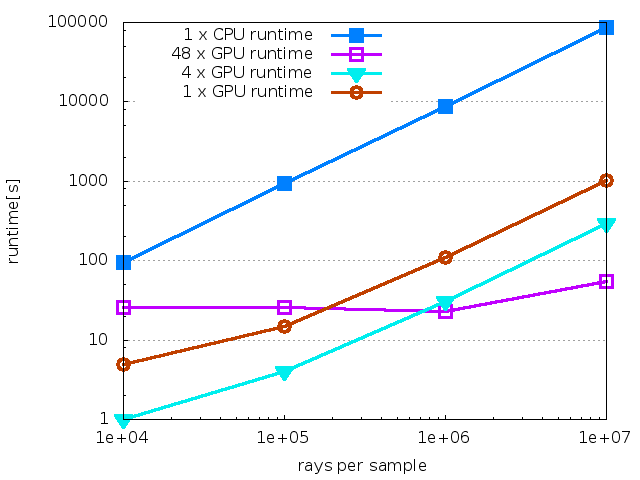
\includegraphics{plot/runtime.png}}}
  \caption{runtime of orginial algorithm compared to parallel algorithm}
  \label{plot:runtime}
\end{figure}
Distributing the computation to multiple devices scales well up to the
point, that every sample point is simulated with the exact same number
of rays. Changing this (e.g. through adaptive sampling), leads to
a potencial unbalanced distribution of computation and therefore to
a worse scaling (figure \ref{plot:gpu_scaling}).
\begin{figure}[H]
  \centerline{
    \resizebox{0.5\textwidth}{!}{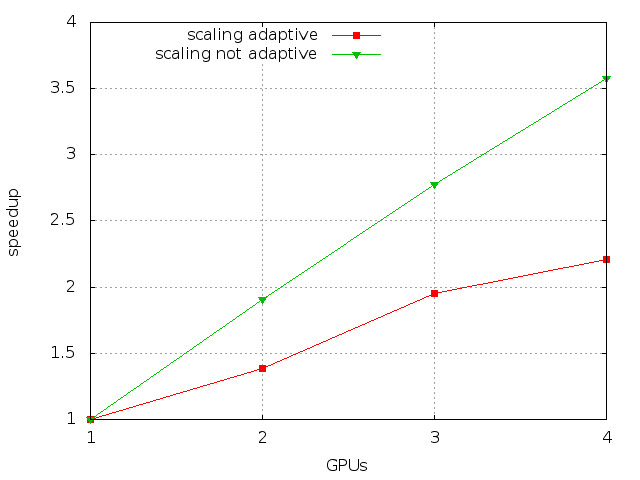
\includegraphics{plot/scaling.png}}}
  \caption{Scaling on multiple devices}
  \label{plot:gpu_scaling}
\end{figure}
But nevertheless, by introducing adaptive sampling, the precision of the the simulation
can be adjusted by a $MSE$-threshold rather than increasing the number
of rays for every sample point. Thus very low computation time results in
simulation values comperable to extremly long simulations (figure \ref{plot:adaptive_runtime})\\
%Please consider, to lower the MSE-Threshold below a certain
%values, exponentially more rays are required.
\begin{figure}[H]
  \centerline{
    \resizebox{0.5\textwidth}{!}{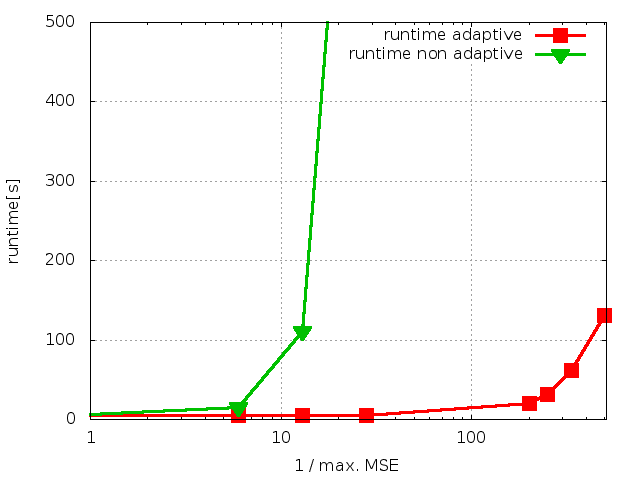
\includegraphics{plot/adaptive_runtime.png}}}
  \caption{runtime comparison of adaptive vs. not adaptive }
  \label{plot:adaptive_runtime}
\end{figure}

\textbf{TODO: FIX MSE BUG}

